\section{Heat Sources and Flames}

\begin{multicols}{2}


\section*{Heat Sources} \index{Heat sources}


\begin{description*}
%\item[Subtopic:]{}
\item[Materials:]{Candle, bottle cap, kerosene burner, tin cans, wire, charcoal, glass jar, metal tubes}
%\item[Setup:]{}
\item[Procedure:]{Construct the simple heat sources shown below.}
%\item[Hazards:]{}
\item[Questions:]{What are the advantages and disadvantages of each?}
%\item[Observations:]{}
%\item[Theory:]{}
%\item[Applications:]{}
%\item[Notes:]{}
\end{description*}

\subsection{Candle Burner}

\begin{center}
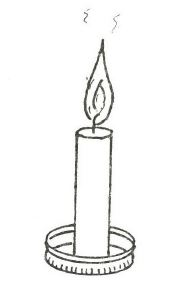
\includegraphics[width=0.1\textwidth]{./img/source/candle-burner.jpg}
\end{center}

\subsection{Kerosene Burner}

\begin{center}
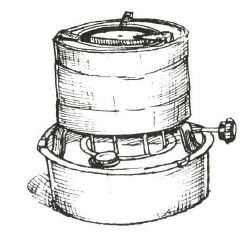
\includegraphics[width=0.3\textwidth]{./img/source/kerosene-burner.jpg}
\end{center}

\subsection{Spirit Burner}

\begin{center}
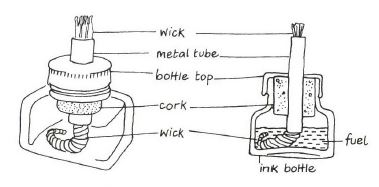
\includegraphics[width=0.49\textwidth]{./img/vso/spirit-burner.jpg}
\end{center}

\vfill
\columnbreak

\subsection{Charcoal Burner}

\begin{center}
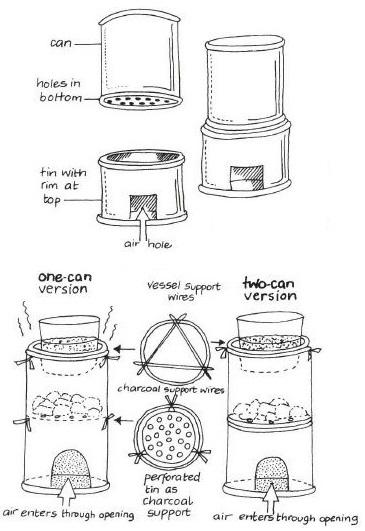
\includegraphics[width=0.49\textwidth]{./img/vso/charcoal-burner.jpg}
\end{center}

\subsection{Types of Flames} \index{Flames}

%\begin{center}
%\includegraphics[width=0.4\textwidth]{./img/.png}
%\end{center}

\begin{description*}
%\item[Subtopic:]{}
\item[Materials:]{Kerosene burner, candle, methylated spirit, kerosene, motopoa, bottle caps, matches, spoon, paper, metal jar lid}
%\item[Setup:]{}
\item[Procedure:]{Light a kerosene burner and observe the flame, adjusting the height of the wicks. Light small amounts of methylated spirit and motopoa in separate bottle caps. Light the candle and observe the flame. Light the paper on a metal lid and observe the flame. For each test, hold a metal spoon over the flame and examine for soot.}
%\item[Hazards:]{}
%\item[Questions:]{}
\item[Observations:]{Kerosene produces a luminous flame. A long wick gives a bigger and brighter flame with more soot. Spirit and motopoa produce non-luminous flames and does not produce soot. Candles and burning paper produce a luminous flame and deposit soot on the spoon.}
%\item[Theory:]{}
%\item[Applications:]{}
%\item[Notes:]{}
\end{description*}


%==================================================================================================%


\end{multicols}

\pagebreak